\chapter{Systemarkitektur}\label{Systemarkitektur}
Der er udarbejdet forskellige diagrammer på baggrund af de specificerede systemkrav.  Diagrammerne har til formål at dele systemet op i realiserbare dele for at vise arkitekturen for systemet. 

Arkitekturen beskriver den grundlæggende organisering af Automatisk Ultralydsscanner og opbygningen af dens tilhørende PC Applikation. Systemet er opbygget generisk, så man vil kunne udskifte komponenter som f.eks. Robotarm eller 3D kamera med en anden type eller model. Udskiftning af komponenter vil dog resultere i en anderledes implementering. Der er i diagrammerne designet ud fra, at 3D kamera er af typen Microsoft Kinect 2.0 og Robotarm er en UR10 robot. 

\section{Systemoversigt}
Systemet Automatisk Ultralydsscanner består af en PC applikation, en Ultralydsscanner, en Robotarm af typen Universal Robots UR10, et 3D kamera af typen Microsoft Kinect 2.0, samt et Access Point, af typen D-Link DAP-1160, til forbindelse mellem Robotarm og PC applikation. Der er fem aktører, Robotarm, Ultralydsscanner, 3D kamera, Operatør og Patient, som interagerer med PC Applikation.

Robotarm har en touch skærm, hvorpå Operatør manuelt kan flytte Robotarm, se Robotarms koordinator samt programmere Robotarm. Robotarm er forbundet via et ethernet kabel af typen RJ45 til et Access Point. PC Applikation er forbundet til Access Point med et kabel af samme type. 3D kamera er forbundet til PC Applikation via 3D kameras USB 3.0 kabel. Ultralydsscanner er en seperat enhed, som blot er fastgjort mekanisk på Robotarms yderste led, men indgår i det fulde system Automatisk Ultralydsscanner. Ultralydsscanner skal manuelt tændes og slukkes af Operatør.

For Automatisk Ultralydsscanner er der udarbejdet forskellige diagrammer, som har til formål at dele systemet op i blokke og vise integration mellem blokkene, samt forbindelser mellem aktører. Diagrammerne vil blive gennemgået nedenfor. 
\newpage

\subsection{Domænemodel}
Domænemodellen på Figur \ref{domain} viser forbindelserne mellem de forskellige aktører i systemet. 

\begin{figure}[H]
    \centering
    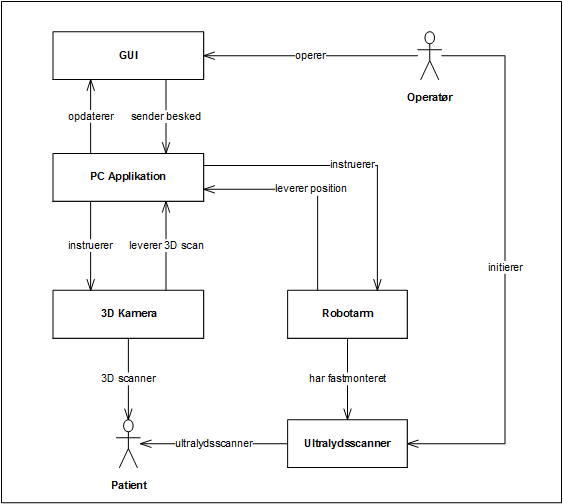
\includegraphics[width=0.7\textwidth]{figurer/d/Design/uml_domain}
    \caption{Domænemodel for Automatisk Ultralydsscanner}
    \label{domain}
\end{figure}

\subsection{Block Definition Diagram}
Block Definition Diagram Figur \ref{BDD} giver et overblik over Automatisk Ultralydsscanners komponenter, som et samlet system.
Her ses, at det er nødvendigt at have en computer med mus og skærm for at anvende PC Applikation.

\begin{figure}[H]
    \centering
    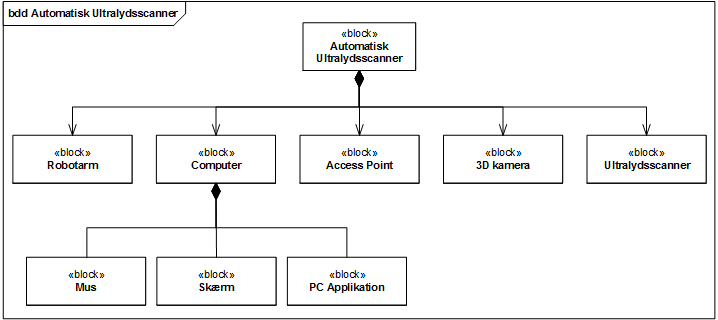
\includegraphics[width=1\textwidth]{figurer/d/Design/BDD}
    \caption{BDD for Automatisk Ultralydsscanner}
    \label{BDD}
\end{figure}
\newpage

\subsection{Internal Block Diagram}
Internal Block Diagram Figur \ref{IBD} viser flow af information mellem de forskellige blokke i Automatisk Ultralydsscanner.
Bemærk at Ultralydsscanner ikke er med, da den ikke interagerer med resten af Automatisk Ultralydsscanner, men blot er forbundet mekanisk til Robotarm.
Når 3D Scan menuen åbnes i PC Applikation, vil der være et konstant flow af dybdedata fra 3D kamera til PC Applikation.
Når PC Applikation startes, vil der være et flow af data frem og tilbage mellem Robotarm og PC Applikation, hvor Access Point agerer som mellemled. 
Forbindelsen mellem PC Applikation og Access Point, samt forbindelsen mellem Access Point og Robotarm er oprettet med ethernet-kabler af typen RJ45.
Forbindelsen mellem PC Applikation og 3D kamera er oprettet med 3D kameras USB 3.0 kabel. 

\begin{figure}[H]
    \centering
    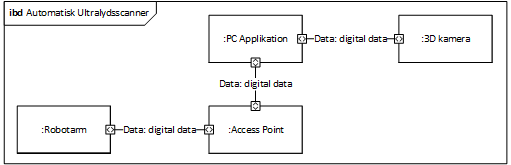
\includegraphics[width=1\textwidth]{figurer/d/Design/IBD}
    \caption{IBD for Automatisk Ultralydsscanner}
    \label{IBD}
\end{figure}

\section{Systemets grænseflader}
Systemet består af to grænseflader: Mellem PC Applikation og Kinect, og mellem PC Aplikation og UR10. Kommunikationen mellem PC Applikation og UR10 sker over modbus-protokollen, hvor kommunikationen mellem PC Applikation og Kinect er gennem Kinect's API via USB.

\subsection{UR10}
Overførsel af data til UR10 sker gennem Transmission Control Protocol/IP-protokollen (TCP/IP). Til afsendelse af positur-værdier fra PC Applikation anvendes modbus-protokollen. Modbus-protokollen sørger for at skrive binære værdier på registre på UR10-controlleren. UR10 kører på URScripts, hvis den skal styres automatisk. UR10 har et script der i en uendelig løkke læser værdierne på registrene og instruerer UR10s Tool Center Point (TCP) til at flytte sig til en positur med en given acceleration og hastighed.

\subsubsection{TCP/IP}
PC Applikation skriver til UR10 over en TCP/IP forbindelse på en IP. Der anvendes to porte; port 502 for kommunikation over modbus-protokollen, og port 30002 for indlæsning af nuværende værdier.
Kommunikationen over port 502 er både read og write, hvor port 30002 kun er read. 
Bemærk, at forskellen  ligger i at de værdier der bliver overført på port 502 kun er til styring af UR10 på script-niveau, som fx den ønskede positur, hastighed og acceleration. Modsat, på port 30002, indhentes de nuværende tilstandsværdier som UR10 har, som fx posituren den reélt har, som ikke nødvendigvis er den samme som den sidste ønskede positur.
For at give et eksempel på hvordan dette foregår sekvensmæssigt:
PC Applikation sender en positur over port 502. Værdierne i denne positur indskrives på UR10s registre.
URScriptet aflæser disse værdier og instruerer UR10 i at flytte sit TCP til denne positur.
Efter noget tid vil den have nået denne positur. Der vil løbende kunne aflæses om UR10 har nået posituren på port 30002.

\textbf{Port 502}
Der er mulighed for at sende informationer om hvor Robotarm skal bevæge sig hen over denne port. For detaljeret specifikation om port 502 og port 30002 henvises der til TRU's dokumentation (\ref{TRUDokumentation}) styk 2.3.2 på side 6.

\textbf{Port 30002}
Der er mulighed for at hive informationer om stort set alle Robotarms nuværende tilstande som fx software version, ledrotationshastighed, tryk feedback m.m. I implementeringen anvendes der kun TCPs rotation og position.

\textbf{URScript} \newline
Scriptet der kører på UR10 aflæser i alt 3 værdier:
Acceleration, hastighed og positur.
Positur består af værdierne X, Y og Z for position og RX, RY og RZ for rotation.
Positur-værdierne aflæses på registrene 135-140 og indsættes som properties i et 'pose' objekt.
Accelerationsværdien, hastighedsværdien samt pose-objektet gives som parameter til funktionen \textit{movel}.
UR10s TCP flyttes lineært i funktionen \textit{move1}. Tiden på acceleration og deceleration styres omvendt proportionalt af accelerationsværdien, mens den maksimale hastighed styres af hastighedsværdien. Se figur \ref{ur10velocity} for et billede af dette. Se manuelen for UR10 (bilag \ref{UserManualUR10}) s. II-48 til II-50 for mere information om \textit{movel}-kommandoen.

\begin{figure}[H]
    \centering
    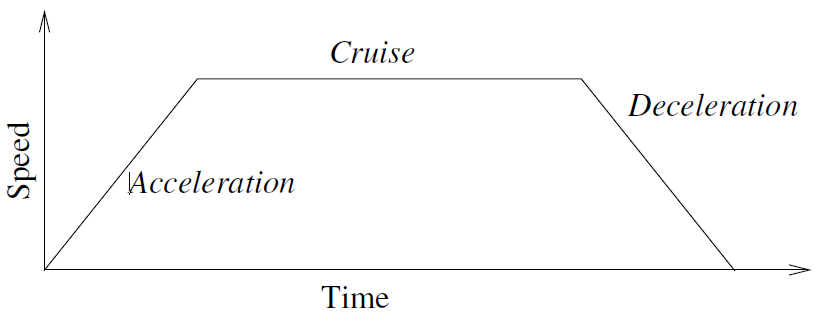
\includegraphics[width=1\textwidth]{figurer/d/movel_velocity}
    \caption{Hastighed over tid som vist i UR10s brugermanuel}
    \label{ur10velocity}
\end{figure}


\subsection{Kinect}
Computeren er forbundet til 3D kamera via USB af typen Transcend PDU3 USB-adapter PCIe 2.0 USB 3.0 eller anden USB3.0 type, der er kompatible med Microsoft Kinect 2.0. 3D kamera har også et supplerende strømforsyningskabel.
For kommunikation med 3D kamera er der brugt Microsoft's Kinect API \cite{KinectAPI} .
Der er taget udgangspunkt i Fusion-delen \cite{KinectFusion} af API'et. Fordelen med dette API er at det kan gøre en masse arbejde - ulempen er at det ikke er generisk. Altså ville man ikke kunne bruge en anden sensor en Microsoft Kinect for Windows 2.0. API'et har en C\#-wrapper, og Microsoft har leveret kildekode til et projekt der gjorde nogenlunde det vi var interesserede i (se reference \cite{KinectFusionExplorer}) for at få den nyeste version af dette.
Efter oprettelsen af forbindelse til Kinect-sensoren er det muligt at 'lytte' på den og få de depth frames den kontinuerligt leverer. Se beskrivelsen af sekvensdiagrammet 3D scan (figur \ref{sd_3Dscan}) i Systemdesign for yderligere forklaring.

\newpage

\section{Softwarearkitektur}
PC Applikation er opdelt af forskellige moduler for at øge samhørigheden og nedsætte koblingen, hvilket er med til at sikre overskuelighed og gøre PC Applikation lettere at vedligeholde og genbruge. Modulerne er inddelt efter ansvarsområder angående præsentation til bruger, kommunikation til Robotarm, indhentning af 3D scan fra 3D kamera samt udregning af Robotarms sti til ultralydsscanning. Disse 4 moduler har fælles datastrukturer. For at undgå cykliske forbindelser, er disse datastrukturer tilføjet til deres eget modul. Figur \ref{Layers} viser referencen mellem modulerne. 

\begin{figure}[H]
    \centering
    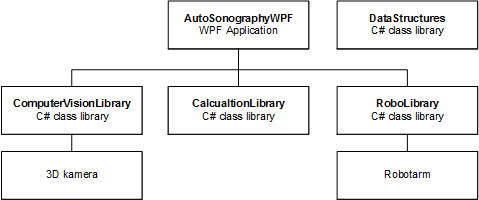
\includegraphics[width=0.75\textwidth]{figurer/d/Design/Layers}
    \caption{PC Applikations opdeling af moduler}
    \label{Layers}
\end{figure}


\begin{table}[htb]
\begin{tabular}{ | l | p{0.7\textwidth} | }
\hline
\textbf{Lag} & \textbf{Beskrivelse af ansvar} \\\hline
AutoSonographyWPF & Håndterer Operatørs interaktion med PC Applikation, hvor Operatør kan vælge 3D scan- eller ultralydsscan. Dette projekt virker som en grænseflade til resten af PC Applikation.\\\hline
ComputerVisionLibrary & Indhenter og afgrænser 3D scanning fra 3D kamera. \\\hline
CalculationLibrary & Sørger for at konvertere en 3D scanning til en sti af positurer som Robotarm kan gennemløbe. \\\hline
RoboLibrary & Muliggør at kommunikere med og instruere Robotarm.\\\hline
DataStructures & Indeholder forskellige data transfer objekter (DTO), der bruges gennem PC Applikation til at sende objekter mellem de forsellige moduler, samt udvidelsesmetoder til eksisterende .NET eller KinectAPI datastrukturer.\\\hline
\end{tabular}
\caption{Modulopdeling og ansvar}
\end{table}

\newpage
\subsection{Pakkediagram}
Pakkediagrammet figur \ref{Pakkediagram} giver en oversigt over afhængighederne i PC Applikation.
For at undgå cykliske forbindelser blev adskillige datastrukturer flyttet fra CalculationLibrary, ComputerVisionLibrary og RoboLibrary til DataStructures-biblioteket.
DataStructures indeholder altså kun nogle datastrukturer og nogle extension-metoder til disse. 
For forklaringen af indholdet af de øvrige pakker, se klassediagrammerne for hvert bibliotek.

\textbf{AutoSocograophyWPF} inderholder alt, der hører til PC Applikations grafiske brugergrænseflade (GUI).

\textbf{ComputerVisionLibrary} indeholder klasser, der interagerer med 3D kamera og udvinder en 3D scanning i et begrænset område.

\textbf{RoboLibray} indeholder klasser som der muliggør kommunikation med Robotarm. 

\textbf{DataStructures} indeholder datastrukturer der bruges på tværs af PC Applikation og nogle extension-metoder til disse. 

\textbf{CalculationLibrary} indeholder klasser der finder stien af positurer i en 3D scanning der er nødvendige for at foretage en ultralydsscanning med Robotarm.

\begin{figure}[H]
    \centering
    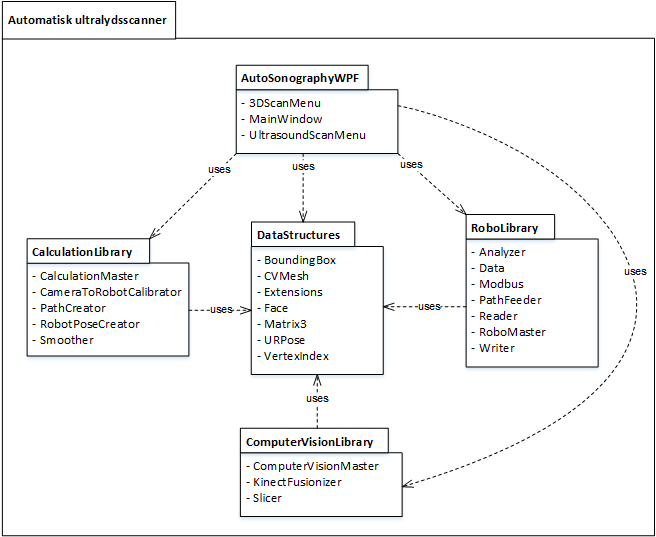
\includegraphics[width=0.9\textwidth]{figurer/d/Design/Pakkediagram}
    \caption{Pakkediagram for Automatisk Ultralydsscanner}
    \label{Pakkediagram}
\end{figure}
\newpage
